\documentclass{article}

\usepackage{tikz}
\usepackage{subcaption}
\usepackage{listings}

\begin{document}

\pagestyle{empty}

\def\layersep{3.5cm}

\section{Task 2}


\subsection{Problem Description}
Instead of trying to find the minimum of the Rosenbrock's function in task 1, we would like to solve the "exclusive or" (xor) problem in task 2. The problem exists out of two input bits which should produce their associated value of the (only) output bit. Please see Table~\ref{tab:tt} for the truth table.

\begin{table}[!h]
	\centering
	\begin{tabular}{| l | c | r |}
		\hline
		$x_1$ & $x_2$ & $y$ \\ \hline
		0 & 0 & 0 \\ \hline
		0 & 1 & 1 \\ \hline
		1 & 0 & 1 \\ \hline
		1 & 1 & 1 \\ \hline
	\end{tabular}
	\caption{The truth table. When only one of the two input bits is true, the output bit should be true.}
	\label{tab:tt}
\end{table}

A perceptron cannot solve this problem, because the classes (different values of y) could not be separated linearly with one line in twodimensional space. Please see Figure~\ref{fig:sep} why. 

\begin{figure}[!h]
	\centering
	\begin{subfigure}[b]{0.3\textwidth}
		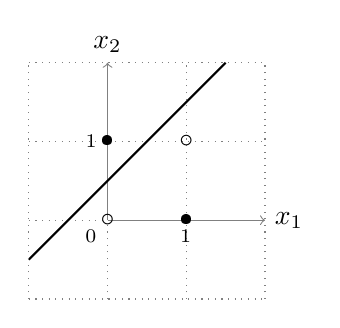
\begin{tikzpicture}[x=1cm,y=1cm]
			\draw[latex-latex, thin, draw=gray, ->] (0,0)--(2,0) node [right] {$x_1$};
			\draw[latex-latex, thin, draw=gray, ->] (0,0)--(0,2) node [above] {$x_2$}; 
			\draw[thick] (-1, -0.5)--(1.5, 2); 

			\draw [dotted, gray] (-1, -1) grid (2, 2);
			\node [black] at (0, 1) {\textbullet};
			\node [black] at (-0.2, 1) {$_1$};
			\node [black] at (1, 0) {\textbullet};
			\node [black] at (1, -0.2) {$_1$};
			\node [black] at (0, 0) {$\circ$} node [below left] {$_0$};
			\node [black] at (1, 1) {$\circ$};
		\end{tikzpicture}
		\caption{}
	\end{subfigure}
	\begin{subfigure}[b]{0.3\textwidth}
		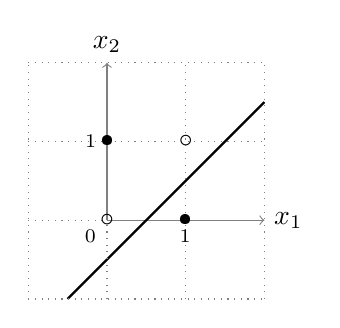
\begin{tikzpicture}[x=1cm,y=1cm]
			\draw[latex-latex, thin, draw=gray, ->] (0,0)--(2,0) node [right] {$x_1$};
			\draw[latex-latex, thin, draw=gray, ->] (0,0)--(0,2) node [above] {$x_2$}; 
			\draw[thick] (-0.5,-1)--(2, 1.5);

			\draw [dotted, gray] (-1, -1) grid (2, 2);
			\node [black] at (0, 1) {\textbullet};
			\node [black] at (-0.2, 1) {$_1$};
			\node [black] at (1, 0) {\textbullet};
			\node [black] at (1, -0.2) {$_1$};
			\node [black] at (0, 0) {$\circ$} node [below left] {$_0$};
			\node [black] at (1, 1) {$\circ$};
		\end{tikzpicture}
		\caption{}
	\end{subfigure}
	\begin{subfigure}[b]{0.3\textwidth}
		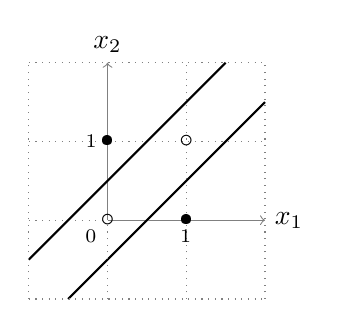
\begin{tikzpicture}[x=1cm,y=1cm]
			\draw[latex-latex, thin, draw=gray, ->] (0,0)--(2,0) node [right] {$x_1$};
			\draw[latex-latex, thin, draw=gray, ->] (0,0)--(0,2) node [above] {$x_2$}; 
			\draw[thick] (-1, -0.5)--(1.5, 2); 
			\draw[thick] (-0.5,-1)--(2, 1.5);

			\draw [dotted, gray] (-1, -1) grid (2, 2);
			\node [black] at (0, 1) {\textbullet};
			\node [black] at (-0.2, 1) {$_1$};
			\node [black] at (1, 0) {\textbullet};
			\node [black] at (1, -0.2) {$_1$};
			\node [black] at (0, 0) {$\circ$} node [below left] {$_0$};
			\node [black] at (1, 1) {$\circ$};
		\end{tikzpicture}
		\caption{}
	\end{subfigure}
	\caption{3 trials to seperate the classes. The filled circles are true cases and the empty circles are false cases.}
	\label{fig:sep}
\end{figure}

As seen in Figure~\ref{fig:sep} (c) it is possible to solve the xor problem, but not with a perceptron. We need something advanced, like a neural network.

\begin{figure}[h]
	\begin{tikzpicture}[shorten >=1pt,->,draw=black!50, node distance=\layersep]
	   	\tikzstyle{every pin edge}=[<-,shorten <=1pt]
		\tikzstyle{neuron}=[circle,fill=black!25,minimum size=17pt,inner sep=0pt]
		\tikzstyle{input neuron}=[neuron, fill=green!50];
		\tikzstyle{output neuron}=[neuron, fill=red!50];
	   	\tikzstyle{hidden neuron}=[neuron, fill=blue!50];
		\tikzstyle{annot} = [text width=4em, text centered]

		% Draw the input layer nodes
		\node[input neuron, pin=left:$x_1$] (I-1) at (0,-1) {};
		\node[input neuron, pin=left:$x_2$] (I-2) at (0,-3) {};

		\path node[hidden neuron] (H-1) at (\layersep,-1 cm) {};
		\path node[hidden neuron] (H-2) at (\layersep,-3 cm) {};

	    	% Draw the output layer node %[yshift=0.5cm]
	    	\node[output neuron,pin={[pin edge={->}]right:y}, right of=H-1, yshift=-1.0cm] (O) {};

		% Connect every node in the input layer with every node in the
		% hidden layer.
		\path (I-1) edge node [above] {$w1$} (H-1) ;
		\path (I-1) edge node [pos=0.75, below, sloped] {$w3$} (H-2);
		\path (I-2) edge node [pos=0.75, above, sloped] {$w2$} (H-1);
		\path (I-2) edge node [below] {$w4$} (H-2);

		% Connect every node in the hidden layer with the output layer
		\path (H-1) edge node [above, sloped] {$w5$} (O);
		\path (H-2) edge node [below, sloped] {$w6$} (O);

		% Annotate the layers
		\node[annot,above of=H-1, node distance=1cm] (hl) {Hidden layer};
		\node[annot,left of=hl] {Input layer};
		\node[annot,right of=hl] {Output layer};
	\end{tikzpicture}
	\caption{The xor neural network.}
	\label{fig:nn}
\end{figure}

\subsection{Solution}
We made a multilayer neural network with three nodes and six weights \footnote{The network could be trained much faster when bias nodes are used, but in sight of the assignment there is chosen to do it the hard way and make the problem more difficult.}. Please see Figure~\ref{fig:nn} for an illustration. The network is trained with the data of the truth table and the weights are updated with the algorithms of task 1. The algorithms tries to steer the weights in such a way the errors of the predicted classes and the actual classes are minimized.

\subsection{Implementation}

\begin{figure}[h]
	\begin{lstlisting}[caption={The computation of the output value, based on the input values and the weights.}, captionpos=b, language=matlab, numbers=left, tabsize=4, frame=single, basicstyle=\footnotesize]
	function [y] = xornet(x1, x2, w)
		net1 = w(1) * x1 + w(2) * x2;
	 	y1 = phi(net1);
		net2 = w(3) * x1 + w(4) * x2;
	 	y2 = phi(net2);
		net = w(5) * y1 + w(6) * y2;
	 	y = phi(net);
	end
	\end{lstlisting}
\end{figure}

The xornet function computes the output value. The ($\phi$) sigmoid function is used as the activation function, so the output value will always lay between 0 and 1. The mysse function calculates the sum squared errors of the network. For every scenario of input values (all four combinations of $x_1$ and $x_2$) the computed value is substracted with the actual value (which is found in the truth table). These values are squared and cumulated. The lower the result the better. The dmysse calculates the derivatives, which are used by the 5 algorithms. So check the correctness of this we used the gradchek function of the Netlab toolbox. The results are in Table~\ref{table:gradchek}. The values of the analytic column are computed with the functions mysse (Listing~\ref{listing:mysse}) and dmysse (Listing~\ref{listing:dmysse}). The values of the diffs column are approximated with a central difference formula with a very small step size. The deltas are the difference between the two methods and are very near to 0. The reason for this is because the gradcheck function produces an approximation. 

\begin{figure}
	\centering
	\begin{eqnarray}
	 \phi(x) & = & \frac{1}{1 + e^{-x}} \\
	   \phi'(x) & = & \phi(x)(1 - \phi(x))
	\end{eqnarray}
	\caption{The sigmoid function (1) and the derivative (2).}
\end{figure}

\begin{figure}
	\begin{lstlisting}[caption={The calculation of the sum squared error of the weights.}, label={listing:mysse}, captionpos=b, language=matlab, numbers=left, tabsize=4, frame=single, basicstyle=\footnotesize, breaklines=true]
function [d] = mysse(w)
	d = power(xornet(0, 0, w) - 0, 2) + 
		power(xornet(0, 1, w) - 1, 2) + 
		power(xornet(1, 0, w) - 1, 2) + 
		power(xornet(1, 1, w) - 0, 2);
end
	\end{lstlisting}
\end{figure}


\begin{figure}
	\begin{lstlisting}[caption={The computation of the derivatives of the sum squared error of the weights.}, label={listing:dmysse}, captionpos=b, language=matlab, numbers=left, tabsize=4, frame=single, basicstyle=\footnotesize, breaklines=true, deletekeywords={input, zeros}]
function [d] = dmysse(w)
	d = zeros(1, 6);

	input = [0, 0; 0, 1; 1, 0; 1, 1];
	target = [0, 1, 1, 0];

	for i = 1:4
		net1 = w(1) * input(i, 1) + w(2) * input(i, 2);
		y1 = phi(net1);
		net2 = w(3) * input(i, 1) + w(4) * input(i, 2);
		y2 = phi(net2);
		net = w(5) * y1 + w(6) * y2; 
		y = phi(net);
	
		d(1) = d(1) + (y - target(i)) * phiprime(net) * w(5) * phiprime(net1) * input(i, 1);
		d(2) = d(2) + (y - target(i)) * phiprime(net) * w(5) * phiprime(net1) * input(i, 2);
		d(3) = d(3) + (y - target(i)) * phiprime(net) * w(6) * phiprime(net2) * input(i, 1);
		d(4) = d(4) + (y - target(i)) * phiprime(net) * w(6) * phiprime(net2) * input(i, 2);
		d(5) = d(5) + (y - target(i)) * phiprime(net) * y1;
		d(6) = d(6) + (y - target(i)) * phiprime(net) * y2;
	end
	d = d * 2;
end
	\end{lstlisting}
\end{figure}

\begin{table}[!h]
	\centering
	\begin{tabular}{| l | l | l | l |}
		\hline
		Weight & Analytic & Diffs & Delta \\ \hline
$w_1$ & -0.005010573901061 & -0.005010573955744 & 0.000000000054682 \\ \hline
%  -0.005010573901061 & -0.005010573955744 &  $5.4682*10^{-11}$ \\ \hline
$w_2$ & -0.003205191664670 & -0.003205191778655 & 0.000000000113985 \\ \hline
%  -0.003205191664670 & -0.003205191778655 & $1.13985*10^{-10}$ \\ \hline
$w_3$ & 0.064350036169591 & 0.064350036188543 & -0.000000000018951 \\ \hline
%   0.064350036169591 & 0.064350036188543 & $-0.1.8951*10^{-11}$ \\ \hline
$w_4$ & 0.043391885718938 & 0.043391885751198 & -0.000000000032260 \\ \hline
%   0.043391885718938 & 0.043391885751198 & $-3.2260*10^{-11}$ \\ \hline
$w_5$ & 0.185666714619300 & 0.185666714558330 & 0.000000000060969 \\ \hline
%  0.185666714619300 & 0.185666714558330 & $6.0969*10^{-11}$ \\ \hline
$w_6$ & 0.181319698693786 & 0.181319698588922 & 0.000000000104864 \\ \hline
%  0.181319698693786 & 0.181319698588922 & $1.04864*10^{-10}$ \\ \hline
	\end{tabular}
	\caption{Results of the gradchek function.}
	\label{table:gradchek}
\end{table}

\begin{table}[!h]
	\centering
	\begin{tabular}{| l | l | l | l |}
		\hline
		Weight & Analytic & Diffs & Delta \\ \hline
$w_1$ & -0.0050 & -0.0050 & $5.4682*10^{-11}$ \\ \hline
$w_2$ & -0.0032 & -0.0032 & $1.1398*10^{-10}$ \\ \hline
$w_3$ & 0.06435 & 0.06435 & $-1.8951*10^{-11}$ \\ \hline
$w_4$ & 0.04339 & 0.04339 & $-3.2260*10^{-11}$ \\ \hline
$w_5$ & 0.18566 & 0.18566 & $6.0969*10^{-11}$ \\ \hline
$w_6$ & 0.18131 & 0.18131 & $1.0486*10^{-10}$ \\ \hline
	\end{tabular}
	\caption{Results of the gradchek function.}
	\label{table:gradchek2}
\end{table}

\subsection{Experiments}
We ran all 5 algorithms for 100 iterations, starting from a random point. This is done 100 times to get the averages of the function evaluations, gradient evaluation and the successrate. The relative amount of times an algorithm is successful after 100 iterations is the successrate. An algorithm is succesful when it can predict all four scenarios correct. Listing~\ref{eq:success} gives more details about this definition. The results are in Table~\ref{table:results}. 

\begin{figure}[!h]
	\begin{lstlisting}[caption={Success condition of a set of weights.}, label={eq:success}, captionpos=b, language=matlab, numbers=left, tabsize=4, frame=single, basicstyle=\footnotesize, breaklines=true, deletekeywords={round}]
success = 	round(xornet(0, 0, w)) == 0 & ...
			round(xornet(1, 1, w)) == 0 & ... 
			round(xornet(0, 1, w)) == 1 & ...
			round(xornet(1, 0, w)) == 1;
	\end{lstlisting}
\end{figure}

\begin{table}[!h]
	\centering
	\begin{tabular}{| l | l | l | l | l |}
		\hline
		Function & Evaluation & Gradient evaluation & Runtime (sec) & Successrate \\ \hline
		Gradient descent & 101 & 100 & 2.0 & 0\% \\ \hline
		Gradient descent (line search) & 1700 & 100 & 5.1 & 0\% \\ \hline
		Scaled conjugate gradient & 67 & 121 & 2.3 & 0\% \\ \hline
		Conjugate gradients & 1691 & 72 & 4.6 & 10\% \\ \hline
		Quasi-Newton & 253 & 82 & 2.0 & 13\% \\ \hline
	\end{tabular}
	\caption{Results of the 5 algorithms. All values are averages and rounded.}
	\label{table:results}
\end{table}

Another experiment was to see how well an naive produce will perform. We generated 10 million random weights sets and tested how many of the sets were successful. Only 8 were successful. 

\section{Conclusion}
Neural networks can solve the xor problem. The update function of the weights are important, because they have different performances. The successrate of the Quasi-Newton method is the highest, but how important is the successrate? We only need one solution to solve the problem and one successful set of weights is not better compared to another successful set of weigths. Gradient descent and scaled conjugate cannot solve this problem within the chosen boundaries. The naive approach of generating random solutions can solve the problem, it only takes a while. Note, probably all functions will perform better if we used bias nodes in the neural network.

\end{document}

